% Options for packages loaded elsewhere
\PassOptionsToPackage{unicode}{hyperref}
\PassOptionsToPackage{hyphens}{url}
%
\documentclass[
  ignorenonframetext,
]{beamer}
\usepackage{pgfpages}
\setbeamertemplate{caption}[numbered]
\setbeamertemplate{caption label separator}{: }
\setbeamercolor{caption name}{fg=normal text.fg}
\beamertemplatenavigationsymbolsempty
% Prevent slide breaks in the middle of a paragraph
\widowpenalties 1 10000
\raggedbottom
\setbeamertemplate{part page}{
  \centering
  \begin{beamercolorbox}[sep=16pt,center]{part title}
    \usebeamerfont{part title}\insertpart\par
  \end{beamercolorbox}
}
\setbeamertemplate{section page}{
  \centering
  \begin{beamercolorbox}[sep=12pt,center]{part title}
    \usebeamerfont{section title}\insertsection\par
  \end{beamercolorbox}
}
\setbeamertemplate{subsection page}{
  \centering
  \begin{beamercolorbox}[sep=8pt,center]{part title}
    \usebeamerfont{subsection title}\insertsubsection\par
  \end{beamercolorbox}
}
\AtBeginPart{
  \frame{\partpage}
}
\AtBeginSection{
  \ifbibliography
  \else
    \frame{\sectionpage}
  \fi
}
\AtBeginSubsection{
  \frame{\subsectionpage}
}
\usepackage{amsmath,amssymb}
\usepackage{lmodern}
\usepackage{iftex}
\ifPDFTeX
  \usepackage[T1]{fontenc}
  \usepackage[utf8]{inputenc}
  \usepackage{textcomp} % provide euro and other symbols
\else % if luatex or xetex
  \usepackage{unicode-math}
  \defaultfontfeatures{Scale=MatchLowercase}
  \defaultfontfeatures[\rmfamily]{Ligatures=TeX,Scale=1}
\fi
% Use upquote if available, for straight quotes in verbatim environments
\IfFileExists{upquote.sty}{\usepackage{upquote}}{}
\IfFileExists{microtype.sty}{% use microtype if available
  \usepackage[]{microtype}
  \UseMicrotypeSet[protrusion]{basicmath} % disable protrusion for tt fonts
}{}
\makeatletter
\@ifundefined{KOMAClassName}{% if non-KOMA class
  \IfFileExists{parskip.sty}{%
    \usepackage{parskip}
  }{% else
    \setlength{\parindent}{0pt}
    \setlength{\parskip}{6pt plus 2pt minus 1pt}}
}{% if KOMA class
  \KOMAoptions{parskip=half}}
\makeatother
\usepackage{xcolor}
\newif\ifbibliography
\usepackage{color}
\usepackage{fancyvrb}
\newcommand{\VerbBar}{|}
\newcommand{\VERB}{\Verb[commandchars=\\\{\}]}
\DefineVerbatimEnvironment{Highlighting}{Verbatim}{commandchars=\\\{\}}
% Add ',fontsize=\small' for more characters per line
\usepackage{framed}
\definecolor{shadecolor}{RGB}{248,248,248}
\newenvironment{Shaded}{\begin{snugshade}}{\end{snugshade}}
\newcommand{\AlertTok}[1]{\textcolor[rgb]{0.94,0.16,0.16}{#1}}
\newcommand{\AnnotationTok}[1]{\textcolor[rgb]{0.56,0.35,0.01}{\textbf{\textit{#1}}}}
\newcommand{\AttributeTok}[1]{\textcolor[rgb]{0.77,0.63,0.00}{#1}}
\newcommand{\BaseNTok}[1]{\textcolor[rgb]{0.00,0.00,0.81}{#1}}
\newcommand{\BuiltInTok}[1]{#1}
\newcommand{\CharTok}[1]{\textcolor[rgb]{0.31,0.60,0.02}{#1}}
\newcommand{\CommentTok}[1]{\textcolor[rgb]{0.56,0.35,0.01}{\textit{#1}}}
\newcommand{\CommentVarTok}[1]{\textcolor[rgb]{0.56,0.35,0.01}{\textbf{\textit{#1}}}}
\newcommand{\ConstantTok}[1]{\textcolor[rgb]{0.00,0.00,0.00}{#1}}
\newcommand{\ControlFlowTok}[1]{\textcolor[rgb]{0.13,0.29,0.53}{\textbf{#1}}}
\newcommand{\DataTypeTok}[1]{\textcolor[rgb]{0.13,0.29,0.53}{#1}}
\newcommand{\DecValTok}[1]{\textcolor[rgb]{0.00,0.00,0.81}{#1}}
\newcommand{\DocumentationTok}[1]{\textcolor[rgb]{0.56,0.35,0.01}{\textbf{\textit{#1}}}}
\newcommand{\ErrorTok}[1]{\textcolor[rgb]{0.64,0.00,0.00}{\textbf{#1}}}
\newcommand{\ExtensionTok}[1]{#1}
\newcommand{\FloatTok}[1]{\textcolor[rgb]{0.00,0.00,0.81}{#1}}
\newcommand{\FunctionTok}[1]{\textcolor[rgb]{0.00,0.00,0.00}{#1}}
\newcommand{\ImportTok}[1]{#1}
\newcommand{\InformationTok}[1]{\textcolor[rgb]{0.56,0.35,0.01}{\textbf{\textit{#1}}}}
\newcommand{\KeywordTok}[1]{\textcolor[rgb]{0.13,0.29,0.53}{\textbf{#1}}}
\newcommand{\NormalTok}[1]{#1}
\newcommand{\OperatorTok}[1]{\textcolor[rgb]{0.81,0.36,0.00}{\textbf{#1}}}
\newcommand{\OtherTok}[1]{\textcolor[rgb]{0.56,0.35,0.01}{#1}}
\newcommand{\PreprocessorTok}[1]{\textcolor[rgb]{0.56,0.35,0.01}{\textit{#1}}}
\newcommand{\RegionMarkerTok}[1]{#1}
\newcommand{\SpecialCharTok}[1]{\textcolor[rgb]{0.00,0.00,0.00}{#1}}
\newcommand{\SpecialStringTok}[1]{\textcolor[rgb]{0.31,0.60,0.02}{#1}}
\newcommand{\StringTok}[1]{\textcolor[rgb]{0.31,0.60,0.02}{#1}}
\newcommand{\VariableTok}[1]{\textcolor[rgb]{0.00,0.00,0.00}{#1}}
\newcommand{\VerbatimStringTok}[1]{\textcolor[rgb]{0.31,0.60,0.02}{#1}}
\newcommand{\WarningTok}[1]{\textcolor[rgb]{0.56,0.35,0.01}{\textbf{\textit{#1}}}}
\usepackage{graphicx}
\makeatletter
\def\maxwidth{\ifdim\Gin@nat@width>\linewidth\linewidth\else\Gin@nat@width\fi}
\def\maxheight{\ifdim\Gin@nat@height>\textheight\textheight\else\Gin@nat@height\fi}
\makeatother
% Scale images if necessary, so that they will not overflow the page
% margins by default, and it is still possible to overwrite the defaults
% using explicit options in \includegraphics[width, height, ...]{}
\setkeys{Gin}{width=\maxwidth,height=\maxheight,keepaspectratio}
% Set default figure placement to htbp
\makeatletter
\def\fps@figure{htbp}
\makeatother
\setlength{\emergencystretch}{3em} % prevent overfull lines
\providecommand{\tightlist}{%
  \setlength{\itemsep}{0pt}\setlength{\parskip}{0pt}}
\setcounter{secnumdepth}{-\maxdimen} % remove section numbering
\ifLuaTeX
  \usepackage{selnolig}  % disable illegal ligatures
\fi
\IfFileExists{bookmark.sty}{\usepackage{bookmark}}{\usepackage{hyperref}}
\IfFileExists{xurl.sty}{\usepackage{xurl}}{} % add URL line breaks if available
\urlstyle{same} % disable monospaced font for URLs
\hypersetup{
  pdftitle={Logistic Regression},
  pdfauthor={Jared Cross},
  hidelinks,
  pdfcreator={LaTeX via pandoc}}

\title{Logistic Regression}
\author{Jared Cross}
\date{2023-01-30}

\begin{document}
\frame{\titlepage}

\begin{frame}[fragile]{Winning Elections}
\protect\hypertarget{winning-elections}{}
Let's take another look at the Hibbs data but this time we'll try to
predict the chance of a candidate winning the popular vote.

\begin{Shaded}
\begin{Highlighting}[]
\NormalTok{hibbs }\OtherTok{=} 
\NormalTok{hibbs }\SpecialCharTok{\%\textgreater{}\%} 
  \FunctionTok{mutate}\NormalTok{(}\AttributeTok{won\_pop =} \FunctionTok{ifelse}\NormalTok{(vote}\SpecialCharTok{\textgreater{}=}\DecValTok{50}\NormalTok{, }\DecValTok{1}\NormalTok{, }\DecValTok{0}\NormalTok{))}
\end{Highlighting}
\end{Shaded}
\end{frame}

\begin{frame}{Winning the Popular Vote}
\protect\hypertarget{winning-the-popular-vote}{}
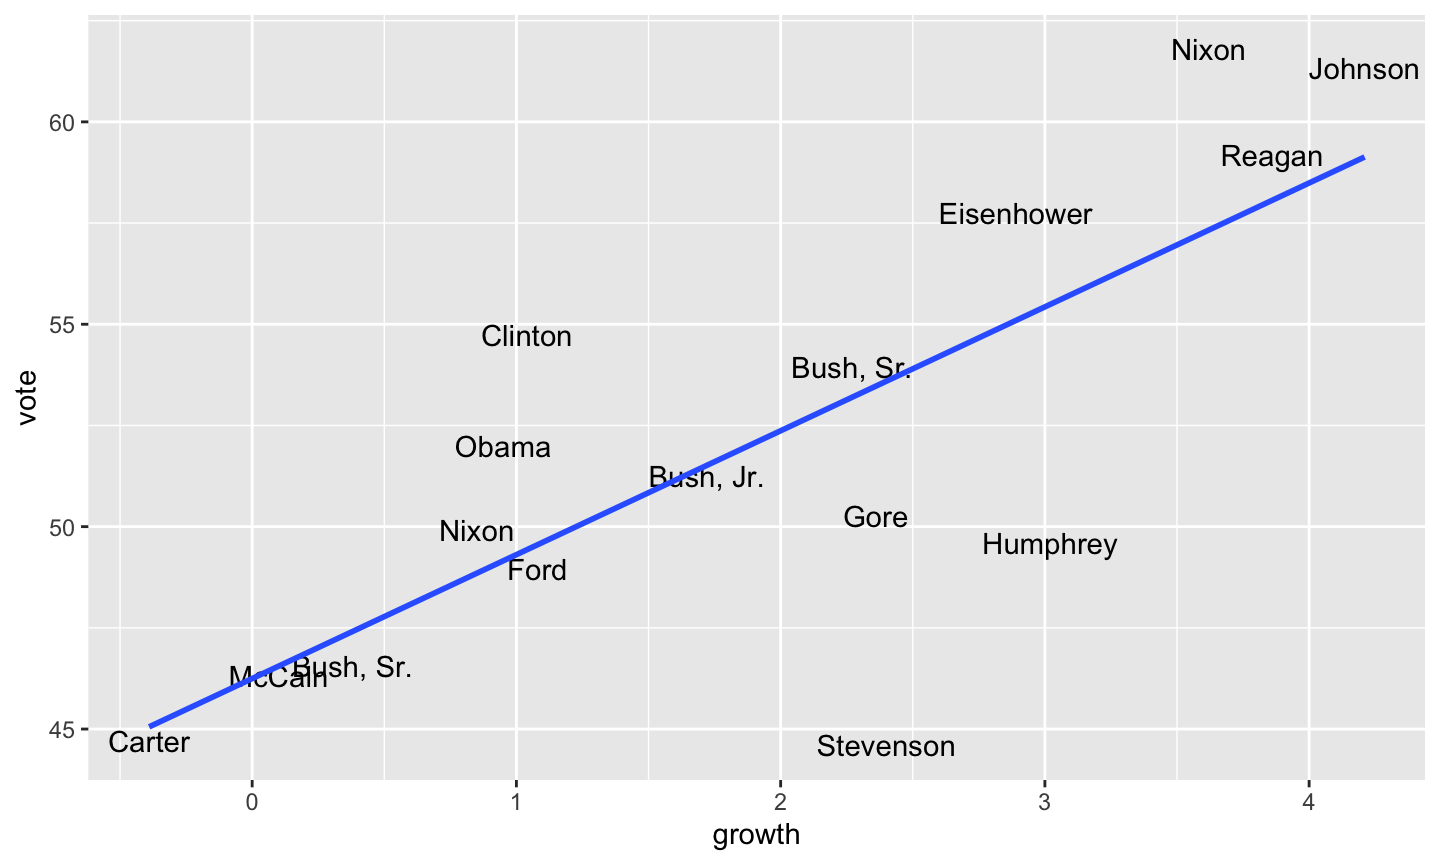
\includegraphics{logistic_regression_files/figure-beamer/unnamed-chunk-3-1.pdf}
\end{frame}

\begin{frame}{Winning the Popular Vote\ldots{}}
\protect\hypertarget{winning-the-popular-vote-1}{}
We can add a best fit line\ldots{}

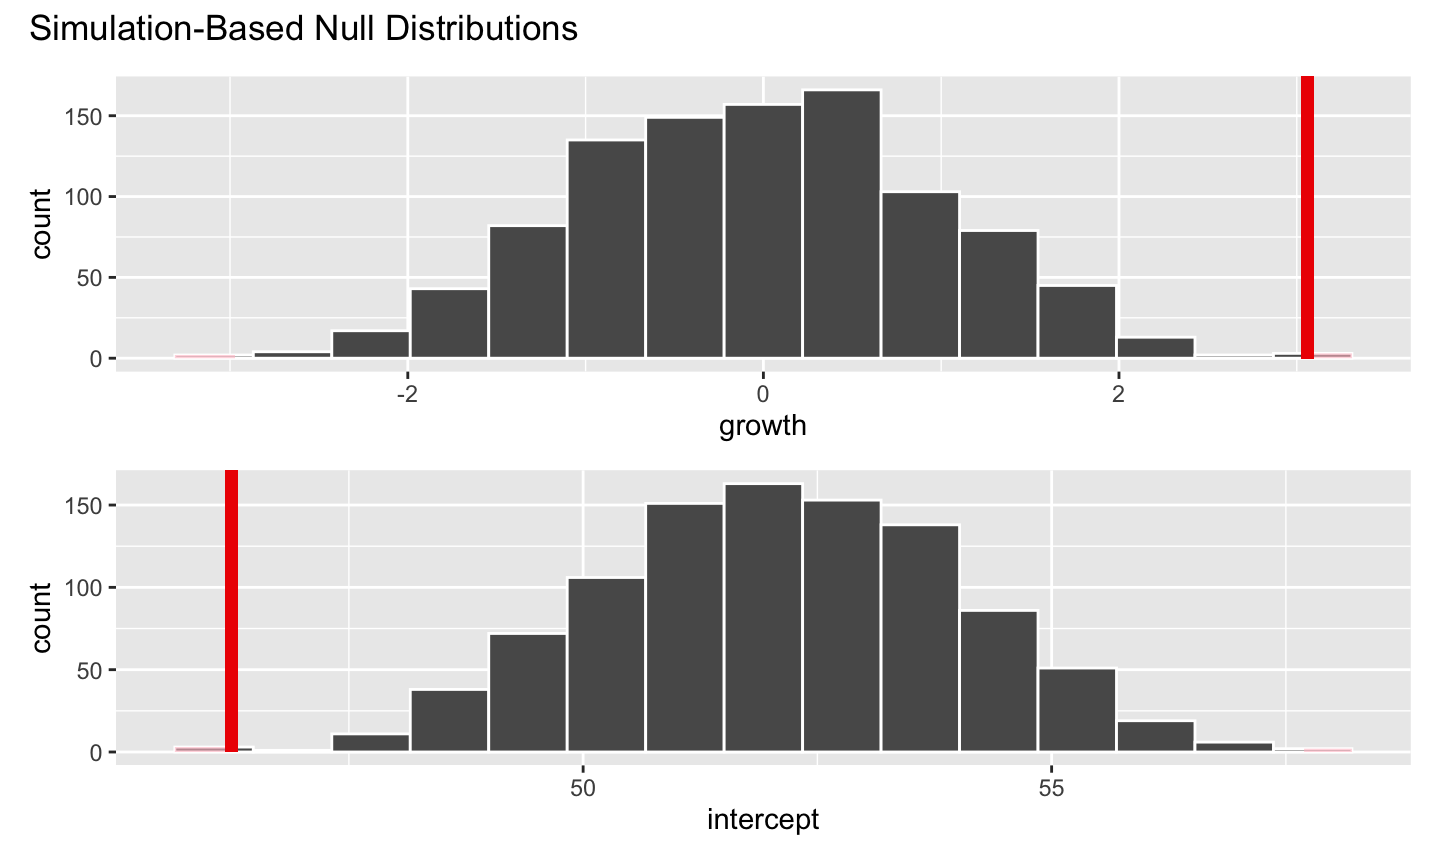
\includegraphics{logistic_regression_files/figure-beamer/unnamed-chunk-4-1.pdf}
\end{frame}

\begin{frame}[fragile]{The Equation (1/2)}
\protect\hypertarget{the-equation-12}{}
\begin{Shaded}
\begin{Highlighting}[]
\NormalTok{m }\OtherTok{=} \FunctionTok{lm}\NormalTok{(won\_pop }\SpecialCharTok{\textasciitilde{}}\NormalTok{ growth, }\AttributeTok{data=}\NormalTok{hibbs)}
\FunctionTok{summary}\NormalTok{(m)}
\end{Highlighting}
\end{Shaded}

\begin{verbatim}
## 
## Call:
## lm(formula = won_pop ~ growth, data = hibbs)
## 
## Residuals:
##      Min       1Q   Median       3Q      Max 
## -0.78700 -0.28250  0.01001  0.34950  0.62700 
## 
## Coefficients:
##             Estimate Std. Error t value Pr(>|t|)  
## (Intercept)  0.18301    0.19167   0.955   0.3559  
## growth       0.20000    0.08228   2.431   0.0291 *
## ---
## Signif. codes:  0 '***' 0.001 '**' 0.01 '*' 0.05 '.' 0.1 ' ' 1
## 
## Residual standard error: 0.4447 on 14 degrees of freedom
## Multiple R-squared:  0.2968, Adjusted R-squared:  0.2465 
## F-statistic: 5.908 on 1 and 14 DF,  p-value: 0.02911
\end{verbatim}
\end{frame}

\begin{frame}{The Equation (2/2)}
\protect\hypertarget{the-equation-22}{}
\[won\_pop = 0.183 + 0.2 \cdot growth\]

\[ 0.183 + 0.2\cdot growth > 1\] \[ 0.2 \cdot growth > 0.717\]
\[ growth > 3.585\]
\end{frame}

\begin{frame}{What if instead\ldots{}}
\protect\hypertarget{what-if-instead}{}
We predict the log odds of winning\ldots{}

\[odds = \frac{probability}{1-probability}\] \[ 0 <= odds <= \infty \]

\[ log\ odds = log(\frac{probability}{1-probability}) \]
\[ -\infty <= log\ odds <= \infty \]
\end{frame}

\begin{frame}[fragile]{Fitting the logistic model}
\protect\hypertarget{fitting-the-logistic-model}{}
Just add a g to lm to make glm: (from linear model to ``generalized''
linear model) Here the family is ``binomial'' (``successes'' and
``failures'')

\begin{verbatim}
## 
## Call:
## glm(formula = won_pop ~ growth, family = "binomial", data = hibbs)
## 
## Deviance Residuals: 
##     Min       1Q   Median       3Q      Max  
## -1.8679  -0.7647   0.3773   0.8479   1.4466  
## 
## Coefficients:
##             Estimate Std. Error z value Pr(>|z|)  
## (Intercept)   -1.608      1.089  -1.476   0.1401  
## growth         1.046      0.544   1.924   0.0544 .
## ---
## Signif. codes:  0 '***' 0.001 '**' 0.01 '*' 0.05 '.' 0.1 ' ' 1
## 
## (Dispersion parameter for binomial family taken to be 1)
## 
##     Null deviance: 21.930  on 15  degrees of freedom
## Residual deviance: 16.581  on 14  degrees of freedom
## AIC: 20.581
## 
## Number of Fisher Scoring iterations: 4
\end{verbatim}
\end{frame}

\begin{frame}{The Logistic Equation}
\protect\hypertarget{the-logistic-equation}{}
\[log\ odds\ prob = -1.608 + 1.046 \cdot growth\]

\[ -1.608 + 1.046 \cdot growth > 0 \] when
\[ 1.046 \cdot growth > 1.608\] \[ growth > 1.54 \]
\end{frame}

\begin{frame}{Plotting the Logistic Equation (1/2)}
\protect\hypertarget{plotting-the-logistic-equation-12}{}
\includegraphics{logistic_regression_files/figure-beamer/unnamed-chunk-7-1.pdf}
\end{frame}

\begin{frame}{Plotting the Logistic Equation (2/2)}
\protect\hypertarget{plotting-the-logistic-equation-22}{}
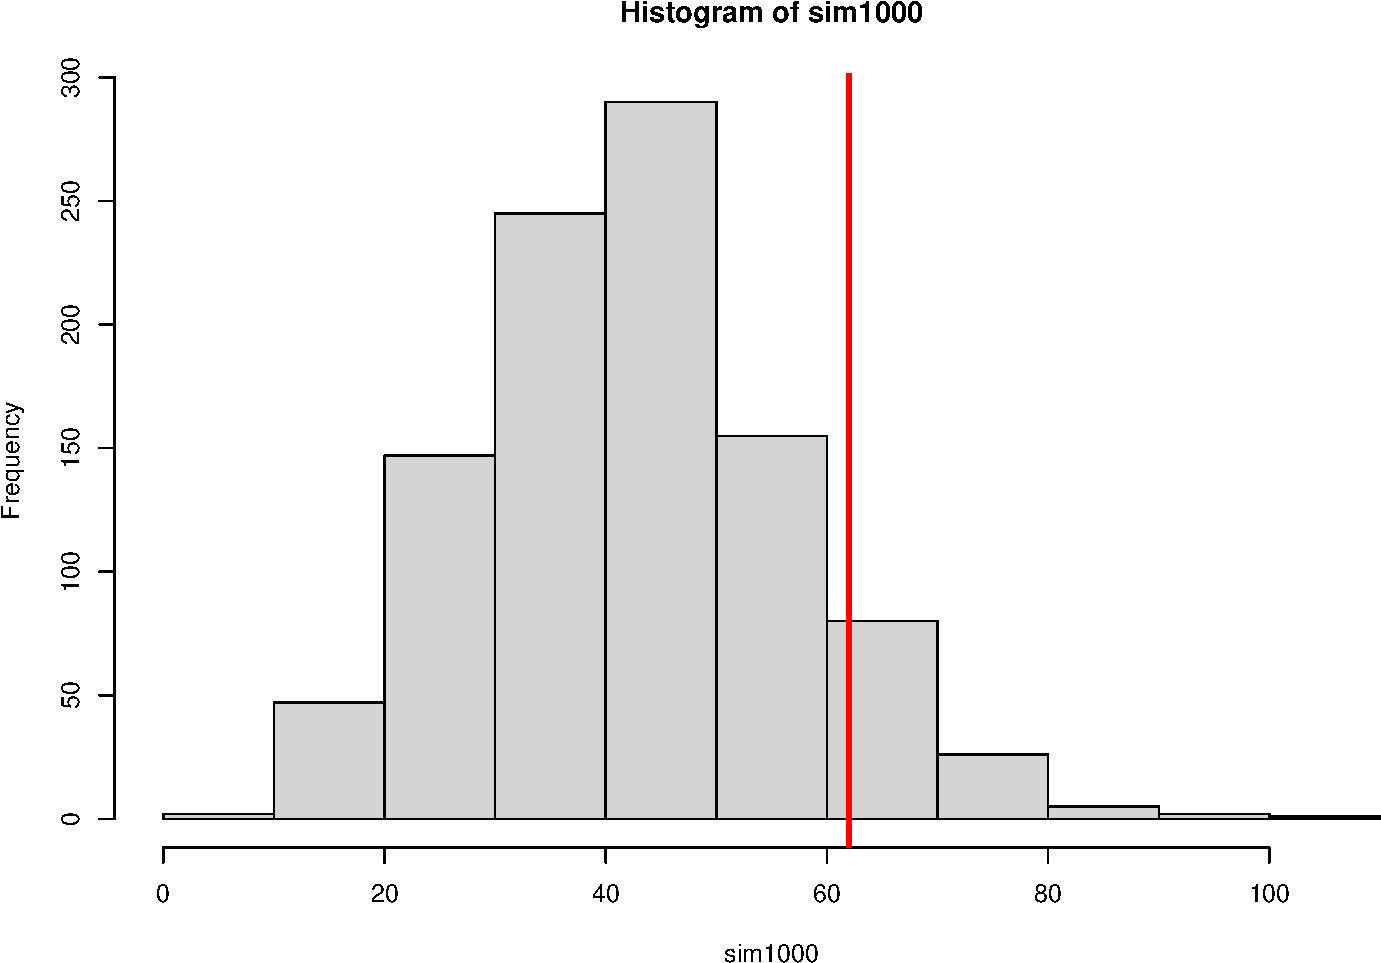
\includegraphics{logistic_regression_files/figure-beamer/unnamed-chunk-8-1.pdf}
\end{frame}

\begin{frame}{The Gory Math}
\protect\hypertarget{the-gory-math}{}
\[log\ odds\ winning = -1.608 + 1.046 \cdot growth\]

\[odds\ winning = e^{-1.608 + 1.046 \cdot growth}\]
\[odds\ winning = e^{-1.608} \cdot e^{1.046 \cdot growth}\]
\[odds\ winning = e^{-1.608} \cdot (e^{1.046})^{growth}\]
\[odds\ winning = 0.2003 \cdot 2.85^{growth}\]

How do we make sense of this?
\end{frame}

\begin{frame}{Logistic Equation Interpretation}
\protect\hypertarget{logistic-equation-interpretation}{}
\[odds\ winning = 0.2003 \cdot 2.85^{growth}\]

With 0\% growth the incumbent party has 0.2 odds of winning (meaning 1
win for every 5 losses). For every additional 1\% growth the incumbents
odds of winning are multiplied by 2.85!

\[ prob\ winning = \frac{0.2003 \cdot 2.85^{growth}}{
1 + 0.2003 \cdot 2.85^{growth}
}\]
\end{frame}

\begin{frame}{Field Goals}
\protect\hypertarget{field-goals}{}
\includegraphics{https://media.giphy.com/media/3oEduNSDOODtlE6CVG/giphy-downsized-large.gif}
\end{frame}

\begin{frame}[fragile]{The Data}
\protect\hypertarget{the-data}{}
\begin{verbatim}
##   Team Year GameMinute Kicker Distance ScoreDiff Grass Success
## 1  PHI 2005          3  Akers       49         0 FALSE       0
## 2  PHI 2005         29  Akers       49        -7 FALSE       0
## 3  PHI 2005         51  Akers       44        -7 FALSE       1
## 4  PHI 2005         14  Akers       43        14  TRUE       0
## 5  PHI 2005         60  Akers       23         0  TRUE       1
## 6  PHI 2005         39  Akers       34        -3  TRUE       1
\end{verbatim}
\end{frame}

\begin{frame}[fragile]{The Data (continued)}
\protect\hypertarget{the-data-continued}{}
\begin{verbatim}
##      Team                Year        GameMinute       Kicker         
##  Length:11187       Min.   :2005   Min.   : 1.00   Length:11187      
##  Class :character   1st Qu.:2007   1st Qu.:19.00   Class :character  
##  Mode  :character   Median :2010   Median :30.00   Mode  :character  
##                     Mean   :2010   Mean   :32.74                     
##                     3rd Qu.:2013   3rd Qu.:46.00                     
##                     Max.   :2015   Max.   :77.00                     
##     Distance      ScoreDiff          Grass            Success      
##  Min.   :18.0   Min.   :-45.0000   Mode :logical   Min.   :0.0000  
##  1st Qu.:28.0   1st Qu.: -4.0000   FALSE:5053      1st Qu.:1.0000  
##  Median :37.0   Median :  0.0000   TRUE :6134      Median :1.0000  
##  Mean   :36.9   Mean   :  0.5843                   Mean   :0.8327  
##  3rd Qu.:45.0   3rd Qu.:  6.0000                   3rd Qu.:1.0000  
##  Max.   :76.0   Max.   : 48.0000                   Max.   :1.0000
\end{verbatim}
\end{frame}

\begin{frame}[fragile]{Plotting the Data (1/3)}
\protect\hypertarget{plotting-the-data-13}{}
\begin{Shaded}
\begin{Highlighting}[]
\NormalTok{kickers }\SpecialCharTok{\%\textgreater{}\%} \FunctionTok{group\_by}\NormalTok{(Distance) }\SpecialCharTok{\%\textgreater{}\%} 
  \FunctionTok{summarize}\NormalTok{(}\AttributeTok{rate =} \FunctionTok{mean}\NormalTok{(Success), }
            \AttributeTok{n=}\FunctionTok{length}\NormalTok{(Success)) }\SpecialCharTok{\%\textgreater{}\%} 
  \FunctionTok{ggplot}\NormalTok{(}\FunctionTok{aes}\NormalTok{(Distance, rate, }\AttributeTok{size=}\NormalTok{n)) }\SpecialCharTok{+} 
  \FunctionTok{geom\_point}\NormalTok{()}
\end{Highlighting}
\end{Shaded}
\end{frame}

\begin{frame}{Plotting the Data (2/3)}
\protect\hypertarget{plotting-the-data-23}{}
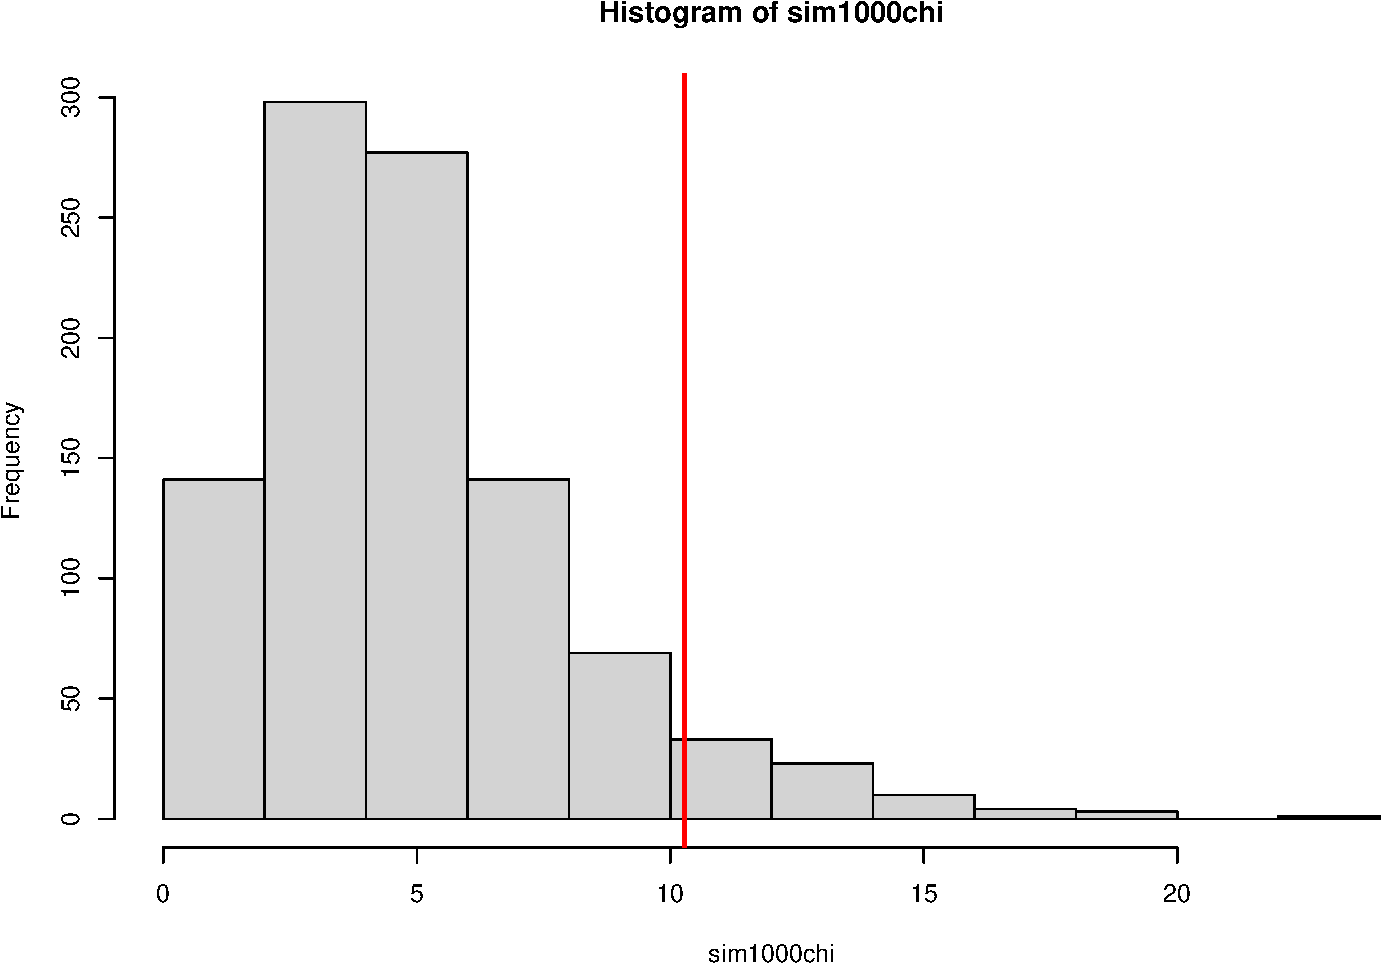
\includegraphics{logistic_regression_files/figure-beamer/unnamed-chunk-12-1.pdf}
\end{frame}

\begin{frame}{Plotting the Data (3/3)}
\protect\hypertarget{plotting-the-data-33}{}
Oh no!!!

\includegraphics{logistic_regression_files/figure-beamer/unnamed-chunk-13-1.pdf}
\end{frame}

\begin{frame}{Logistic Regression?}
\protect\hypertarget{logistic-regression}{}
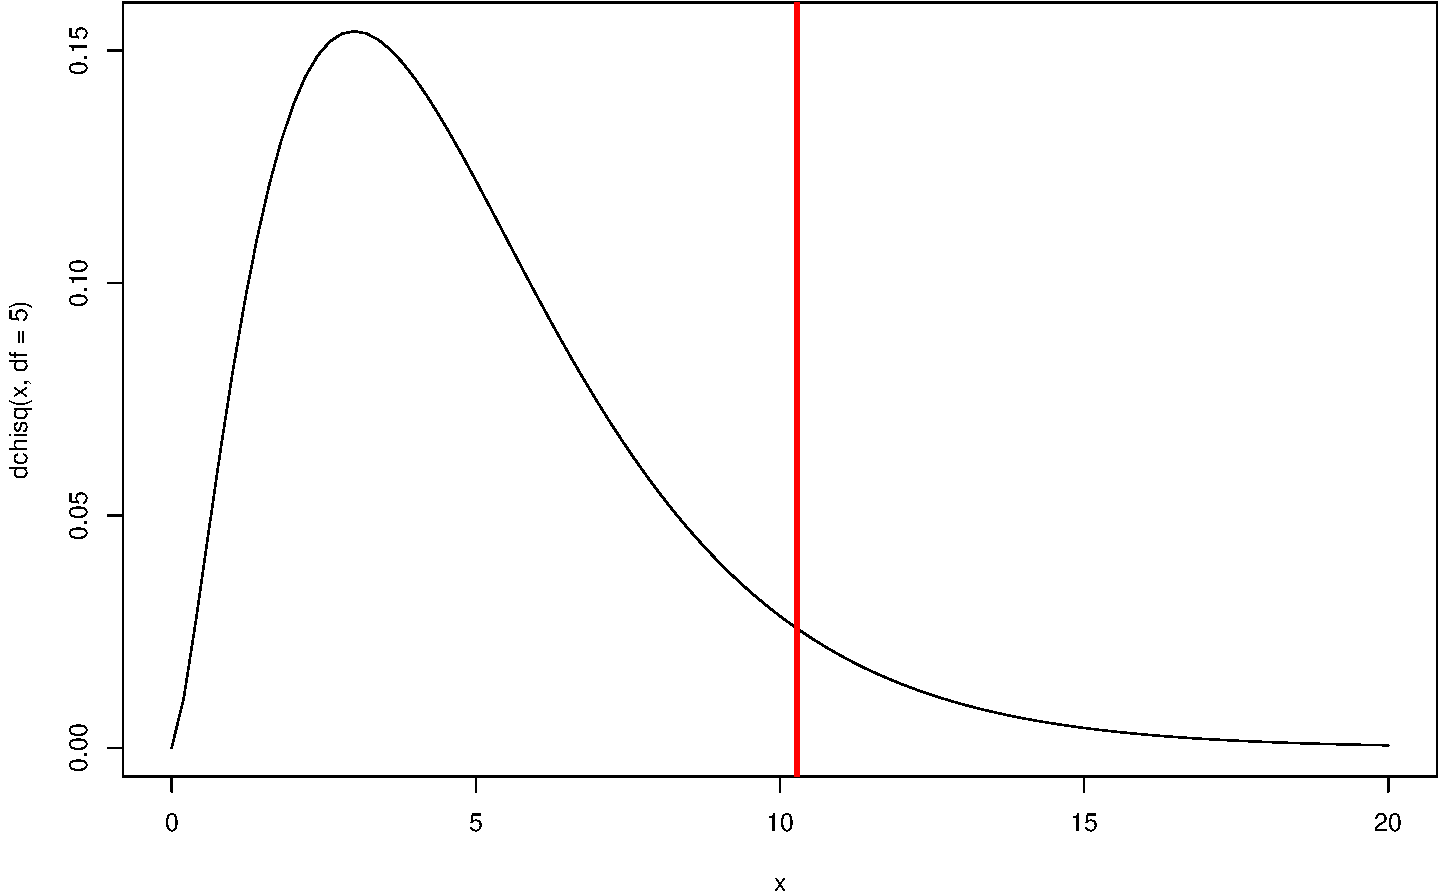
\includegraphics{logistic_regression_files/figure-beamer/unnamed-chunk-14-1.pdf}
\end{frame}

\begin{frame}[fragile]{Fitting the Model}
\protect\hypertarget{fitting-the-model}{}
\begin{Shaded}
\begin{Highlighting}[]
\NormalTok{m.logistic }\OtherTok{\textless{}{-}} \FunctionTok{glm}\NormalTok{(Success }\SpecialCharTok{\textasciitilde{}}\NormalTok{ Distance, }\AttributeTok{data=}\NormalTok{kickers, }\AttributeTok{family=}\StringTok{"binomial"}\NormalTok{)}
\FunctionTok{coef}\NormalTok{(m.logistic)}
\end{Highlighting}
\end{Shaded}

\begin{verbatim}
## (Intercept)    Distance 
##   5.7246196  -0.1026151
\end{verbatim}

\[log\ odds\ success = 5.72 - 0.1026 \cdot Distance\]
\[ odds\ success = e^{5.72 - 0.1026 \cdot Distance}\]

\[ odds\ success = e^{5.72} \cdot (e^{-0.1026})^{Distance} \]

\[ odds\ success = 304.9 \cdot 0.9025^{Distance}\]
\end{frame}

\begin{frame}[fragile]{Interpreting the Model}
\protect\hypertarget{interpreting-the-model}{}
\[304.9 \cdot 0.9025^{Distance} = 1\]

when

\[ 0.9025^{Distance} = 0.003279764\]

\begin{Shaded}
\begin{Highlighting}[]
\FunctionTok{log}\NormalTok{(}\DecValTok{1}\SpecialCharTok{/}\FloatTok{304.9}\NormalTok{, }\AttributeTok{base=}\FloatTok{0.9025}\NormalTok{)}
\end{Highlighting}
\end{Shaded}

\begin{verbatim}
## [1] 55.75762
\end{verbatim}

There are even odds to make a field goal at 56 yards.

The odds get multiple by 0.9 every extra yard or but in half (roughly)
every 7 yards.
\end{frame}

\begin{frame}[fragile]{On Grass or Turf?}
\protect\hypertarget{on-grass-or-turf}{}
Use the following code to find the effect of kicking on grass relative
to kicking on turf.

\begin{Shaded}
\begin{Highlighting}[]
\NormalTok{m.logistic }\OtherTok{\textless{}{-}} \FunctionTok{glm}\NormalTok{(Success }\SpecialCharTok{\textasciitilde{}}\NormalTok{ Distance }\SpecialCharTok{+}\NormalTok{ Grass,}
                  \AttributeTok{data=}\NormalTok{kickers, }\AttributeTok{family=}\StringTok{"binomial"}\NormalTok{)}
\end{Highlighting}
\end{Shaded}
\end{frame}

\begin{frame}[fragile]{Looking at the Grass or Turf Model}
\protect\hypertarget{looking-at-the-grass-or-turf-model}{}
\begin{verbatim}
## 
## Call:
## glm(formula = Success ~ Distance + Grass, family = "binomial", 
##     data = kickers)
## 
## Deviance Residuals: 
##     Min       1Q   Median       3Q      Max  
## -2.7542   0.2486   0.4028   0.6511   1.5849  
## 
## Coefficients:
##              Estimate Std. Error z value Pr(>|z|)    
## (Intercept)  5.825574   0.141694  41.114  < 2e-16 ***
## Distance    -0.102782   0.003139 -32.742  < 2e-16 ***
## GrassTRUE   -0.168174   0.054718  -3.073  0.00212 ** 
## ---
## Signif. codes:  0 '***' 0.001 '**' 0.01 '*' 0.05 '.' 0.1 ' ' 1
## 
## (Dispersion parameter for binomial family taken to be 1)
## 
##     Null deviance: 10105.0  on 11186  degrees of freedom
## Residual deviance:  8738.9  on 11184  degrees of freedom
## AIC: 8744.9
## 
## Number of Fisher Scoring iterations: 5
\end{verbatim}
\end{frame}

\begin{frame}[fragile]{Interpreting the Grass or Turf Model}
\protect\hypertarget{interpreting-the-grass-or-turf-model}{}
\begin{Shaded}
\begin{Highlighting}[]
\FunctionTok{coef}\NormalTok{(m.logistic)}
\end{Highlighting}
\end{Shaded}

\begin{verbatim}
## (Intercept)    Distance   GrassTRUE 
##   5.8255740  -0.1027818  -0.1681737
\end{verbatim}

\[log\ odds\ success = 5.826 -0.103 \cdot Distance -0.168 \cdot Grass\]

\begin{Shaded}
\begin{Highlighting}[]
\FunctionTok{exp}\NormalTok{(}\FunctionTok{coef}\NormalTok{(m.logistic))}
\end{Highlighting}
\end{Shaded}

\begin{verbatim}
## (Intercept)    Distance   GrassTRUE 
## 338.8555700   0.9023238   0.8452070
\end{verbatim}

\[odds\ success = 338.9 \cdot 0.902^{Distance} \cdot 0.845^{Grass}\]

Does Grass affect field goals?
\end{frame}

\begin{frame}{Plotting the Grass or Turf Model}
\protect\hypertarget{plotting-the-grass-or-turf-model}{}
Red is Turf

\includegraphics{logistic_regression_files/figure-beamer/unnamed-chunk-21-1.pdf}
\end{frame}

\begin{frame}[fragile]{Are Kickers Getting Better? (1/3)}
\protect\hypertarget{are-kickers-getting-better-13}{}
\begin{Shaded}
\begin{Highlighting}[]
\NormalTok{m.logistic }\OtherTok{\textless{}{-}} \FunctionTok{glm}\NormalTok{(Success }\SpecialCharTok{\textasciitilde{}}\NormalTok{ Distance}\SpecialCharTok{+}\NormalTok{Grass}\SpecialCharTok{+}\NormalTok{Year,}
                  \AttributeTok{data=}\NormalTok{kickers, }\AttributeTok{family=}\StringTok{"binomial"}\NormalTok{)}
\end{Highlighting}
\end{Shaded}
\end{frame}

\begin{frame}[fragile]{Are Kickers Getting Better? (2/3)}
\protect\hypertarget{are-kickers-getting-better-23}{}
\begin{verbatim}
## 
## Call:
## glm(formula = Success ~ Distance + Grass + Year, family = "binomial", 
##     data = kickers)
## 
## Deviance Residuals: 
##     Min       1Q   Median       3Q      Max  
## -2.7683   0.2456   0.3975   0.6371   1.6056  
## 
## Coefficients:
##               Estimate Std. Error z value Pr(>|z|)    
## (Intercept) -1.042e+02  1.732e+01  -6.017 1.78e-09 ***
## Distance    -1.047e-01  3.175e-03 -32.976  < 2e-16 ***
## GrassTRUE   -1.549e-01  5.488e-02  -2.823  0.00476 ** 
## Year         5.479e-02  8.626e-03   6.352 2.13e-10 ***
## ---
## Signif. codes:  0 '***' 0.001 '**' 0.01 '*' 0.05 '.' 0.1 ' ' 1
## 
## (Dispersion parameter for binomial family taken to be 1)
## 
##     Null deviance: 10105.0  on 11186  degrees of freedom
## Residual deviance:  8698.3  on 11183  degrees of freedom
## AIC: 8706.3
## 
## Number of Fisher Scoring iterations: 5
\end{verbatim}
\end{frame}

\begin{frame}{Are Kickers Getting Better? (3/3)}
\protect\hypertarget{are-kickers-getting-better-33}{}
\includegraphics{logistic_regression_files/figure-beamer/unnamed-chunk-24-1.pdf}
\end{frame}

\begin{frame}{Is there something we could do better?}
\protect\hypertarget{is-there-something-we-could-do-better}{}
\includegraphics{logistic_regression_files/figure-beamer/unnamed-chunk-25-1.pdf}
\end{frame}

\begin{frame}{Trying to Understand What's Going On!}
\protect\hypertarget{trying-to-understand-whats-going-on}{}
Imagine a simpler world where kicks miss for one of two reasons:

\begin{itemize}
\item
  The weren't long enough
\item
  The missed left or right
\end{itemize}

I'll further pretend (for now) that these are independent.

\[P(success) = P(long\ enough)\cdot P(good\ angle)\]
\end{frame}

\begin{frame}{P(long enough)}
\protect\hypertarget{plong-enough}{}
Let's pretend that at Distance = 0 all kicks are long enough and that
P(long enough) goes down with distance but never drops below zero

\[P(long\ enough) = \frac{1}{1 + e^{a + b\cdot Distance}}\] where I
don't know what \textbf{a} and \textbf{b} are.
\end{frame}

\begin{frame}{P(good angle)}
\protect\hypertarget{pgood-angle}{}
The width of the crossbar is about 6 meters, so if kickers aim for the
middle they can miss in either direction by, as long as they miss by
less than 3 meters and still make the kick.

Let's express that acceptable miss as an angle:

\[Acceptable\ Miss\ Angle < sin(\frac{3}{Distance})\]
\end{frame}

\begin{frame}[fragile]{P(good angle) continued}
\protect\hypertarget{pgood-angle-continued}{}
Let's assume that kickers angles are normally distributed around dead
center with a standard deviation of \(\sigma\).

Then the probability of missing is the chance of a z-score more than the
acceptable miss angle.

In other words, if the acceptable miss angle is \(10^{\circ}\) and a
kicker has a standard deviation of \(5^{\circ}\) then the chance of a
good angle is:

\begin{Shaded}
\begin{Highlighting}[]
\FunctionTok{pnorm}\NormalTok{(}\DecValTok{10}\SpecialCharTok{/}\DecValTok{5}\NormalTok{) }\SpecialCharTok{{-}} \FunctionTok{pnorm}\NormalTok{(}\SpecialCharTok{{-}}\DecValTok{10}\SpecialCharTok{/}\DecValTok{5}\NormalTok{)}
\end{Highlighting}
\end{Shaded}

\begin{verbatim}
## [1] 0.9544997
\end{verbatim}

\begin{Shaded}
\begin{Highlighting}[]
\DecValTok{2}\SpecialCharTok{*}\FunctionTok{pnorm}\NormalTok{(}\DecValTok{10}\SpecialCharTok{/}\DecValTok{5}\NormalTok{) }\SpecialCharTok{{-}} \DecValTok{1}
\end{Highlighting}
\end{Shaded}

\begin{verbatim}
## [1] 0.9544997
\end{verbatim}
\end{frame}

\begin{frame}{P(good angle) \ldots{} putting it all together}
\protect\hypertarget{pgood-angle-putting-it-all-together}{}
\[ P(good\ angle) = 2*pnorm(\frac{Largest\ Acceptable\ Miss}{\sigma}) - 1 \]
\[Largest\ Acceptable\ Miss\ Angle = sin(\frac{3}{Distance})\]
\[P(good\ angle) = 2*pnorm(\frac{sin(\frac{3}{Distance})}{\sigma}) - 1\]
\end{frame}

\begin{frame}{P(success)}
\protect\hypertarget{psuccess}{}
\[P(success) = P(long\ enough)\cdot P(good\ angle)\]

\[P(success) = \frac{2*pnorm(\frac{sin(\frac{3}{Distance})}{\sigma}) - 1}{1 + e^{a + b\cdot Distance}}\]
We just need to use the data to solve for \textbf{a}, \textbf{b} and
\textbf{\(\sigma\)}!
\end{frame}

\begin{frame}[fragile]{Nonlinear Least Squares Regression (1/3)}
\protect\hypertarget{nonlinear-least-squares-regression-13}{}
\begin{Shaded}
\begin{Highlighting}[]
\NormalTok{success\_at\_distance }\OtherTok{=} 
\NormalTok{kickers }\SpecialCharTok{\%\textgreater{}\%} \FunctionTok{group\_by}\NormalTok{(Distance) }\SpecialCharTok{\%\textgreater{}\%} 
  \FunctionTok{summarize}\NormalTok{(}\AttributeTok{rate =} \FunctionTok{mean}\NormalTok{(Success), }
            \AttributeTok{n=}\FunctionTok{length}\NormalTok{(Success))}
\end{Highlighting}
\end{Shaded}
\end{frame}

\begin{frame}[fragile]{Nonlinear Least Squares Regression (2/3)}
\protect\hypertarget{nonlinear-least-squares-regression-23}{}
\begin{Shaded}
\begin{Highlighting}[]
\NormalTok{m }\OtherTok{=} \FunctionTok{nls}\NormalTok{(rate }\SpecialCharTok{\textasciitilde{}}\NormalTok{ (}\DecValTok{2}\SpecialCharTok{*}\FunctionTok{pnorm}\NormalTok{(}\FunctionTok{sin}\NormalTok{(}\DecValTok{3}\SpecialCharTok{/}\NormalTok{Distance)}\SpecialCharTok{/}\NormalTok{s)}\SpecialCharTok{{-}}\DecValTok{1}\NormalTok{)}\SpecialCharTok{/}
\NormalTok{              (}\DecValTok{1} \SpecialCharTok{+} \FunctionTok{exp}\NormalTok{(a }\SpecialCharTok{+}\NormalTok{ b}\SpecialCharTok{*}\NormalTok{Distance)),}
               \AttributeTok{start=}\FunctionTok{list}\NormalTok{(}\AttributeTok{s=}\NormalTok{pi}\SpecialCharTok{/}\DecValTok{36}\NormalTok{, }\AttributeTok{a =} \SpecialCharTok{{-}}\DecValTok{9}\NormalTok{, }\AttributeTok{b=}\FloatTok{0.15}\NormalTok{),}
               \AttributeTok{data=}\NormalTok{success\_at\_distance,}
               \AttributeTok{weights=}\NormalTok{n)}
\end{Highlighting}
\end{Shaded}
\end{frame}

\begin{frame}[fragile]{Nonlinear Least Squares Regression (3/3)}
\protect\hypertarget{nonlinear-least-squares-regression-33}{}
\begin{verbatim}
## 
## Formula: rate ~ (2 * pnorm(sin(3/Distance)/s) - 1)/(1 + exp(a + b * Distance))
## 
## Parameters:
##     Estimate Std. Error t value Pr(>|t|)    
## s  5.501e-02  8.479e-04  64.880  < 2e-16 ***
## a -1.386e+01  1.665e+00  -8.327 5.22e-11 ***
## b  2.288e-01  2.993e-02   7.642 5.97e-10 ***
## ---
## Signif. codes:  0 '***' 0.001 '**' 0.01 '*' 0.05 '.' 0.1 ' ' 1
## 
## Residual standard error: 0.3416 on 50 degrees of freedom
## 
## Number of iterations to convergence: 6 
## Achieved convergence tolerance: 7.891e-06
\end{verbatim}
\end{frame}

\begin{frame}{Plotting the Results}
\protect\hypertarget{plotting-the-results}{}
(with the old logistic regression in red)

\includegraphics{logistic_regression_files/figure-beamer/unnamed-chunk-30-1.pdf}
\end{frame}

\begin{frame}{Looking at the Two Factors}
\protect\hypertarget{looking-at-the-two-factors}{}
P(Good Angle) in blue P(Far Enough) in green

\includegraphics{logistic_regression_files/figure-beamer/unnamed-chunk-31-1.pdf}
\end{frame}

\begin{frame}[fragile]{We could keep going!}
\protect\hypertarget{we-could-keep-going}{}
\begin{itemize}
\item
  Maybe kickers angles aren't normally distributed. Are there more
  mishits/outliers than we'd expect based on the normal distribution? If
  so, maybe we need a distribution with fatter tails? What about a
  t-distribution with 3 degrees of freedom?
\item
  What if angles are more unpredictable for longer kicks? This could if
  kickers are less accurate when they try to kick harder or because
  footballs slice or hook.
\end{itemize}

\[ P(good\ angle) = (2\cdot pt(\frac{sin(\frac{3}{Distance})}{\sigma_1+\sigma_2\cdot Distance}, df=3)-1)\]
\#\# The New Model

\begin{Shaded}
\begin{Highlighting}[]
\NormalTok{m2 }\OtherTok{=} \FunctionTok{nls}\NormalTok{(rate }\SpecialCharTok{\textasciitilde{}}\NormalTok{ (}\DecValTok{2}\SpecialCharTok{*}\FunctionTok{pt}\NormalTok{(}\FunctionTok{sin}\NormalTok{(}\DecValTok{3}\SpecialCharTok{/}\NormalTok{Distance)}\SpecialCharTok{/}\NormalTok{(s}\SpecialCharTok{+}\NormalTok{s2}\SpecialCharTok{*}\NormalTok{Distance), }\AttributeTok{df=}\DecValTok{3}\NormalTok{)}\SpecialCharTok{{-}}\DecValTok{1}\NormalTok{)}\SpecialCharTok{/}
\NormalTok{          (}\DecValTok{1} \SpecialCharTok{+} \FunctionTok{exp}\NormalTok{(a }\SpecialCharTok{+}\NormalTok{ b}\SpecialCharTok{*}\NormalTok{Distance)),}
        \AttributeTok{start=}\FunctionTok{list}\NormalTok{(}\AttributeTok{s=}\FloatTok{5.501e{-}02}\NormalTok{, }
                   \AttributeTok{a =} \SpecialCharTok{{-}}\FloatTok{1.386e+01}\NormalTok{, }
                   \AttributeTok{b=}\FloatTok{2.288e{-}01}\NormalTok{,}
                   \AttributeTok{s2=}\DecValTok{0}\NormalTok{),}
        \AttributeTok{data=}\NormalTok{success\_at\_distance,}
        \AttributeTok{weights=}\NormalTok{n)}
\end{Highlighting}
\end{Shaded}
\end{frame}

\begin{frame}{The New Plot}
\protect\hypertarget{the-new-plot}{}
\includegraphics{logistic_regression_files/figure-beamer/unnamed-chunk-33-1.pdf}
\end{frame}

\end{document}
